\chapter{Tecnología de Circuito Integrado}

\section{Tecnología de Circuito Integrado}
\subsection{Tecnología bipolar BJT}

\begin{figure}[H]
    \centering
    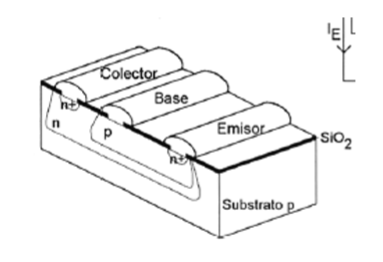
\includegraphics[width=0.5\linewidth]{Imagenes/Tecnologia de CI - BJT.png}
\end{figure}

Proceso de fabricación:

\begin{enumerate}
    \item Predeposición de la capa n+ (capa enterrada)
    \item Crecimiento epitaxial tipo n
    \item Difusión tipo p de aislamiento del transistor
    \item Difusión de tipo p del terminal de base
    \item Predeposición de tipo n+ del terminal de emisor y contacto óhmico del colector
    \item Recubrimiento por crecimiento eopitaxial de capa de SiO2
    \item Apertura fotolitográfica para acceder a los terminales de E, B y C.
    \item Deposición de las metalizaciones de E, B y C.
\end{enumerate}

\subsection{Transistor JFET}

\begin{figure}[H]
    \centering
    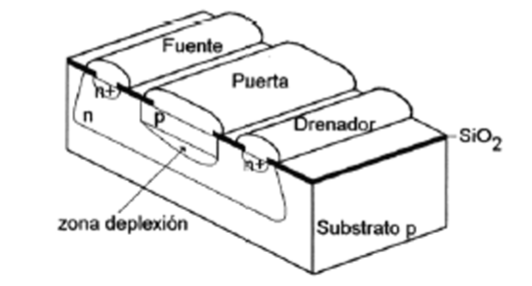
\includegraphics[width=0.5\linewidth]{Imagenes/Tecnologia de CI - JFET.png}
\end{figure}

\begin{enumerate}
    \item Creación zona tipo n
    \item Zona de tipo p
    \item Zona de tipo n+
\end{enumerate}

\subsection{Tecnología MOSFET}

\begin{figure}[H]
    \centering
    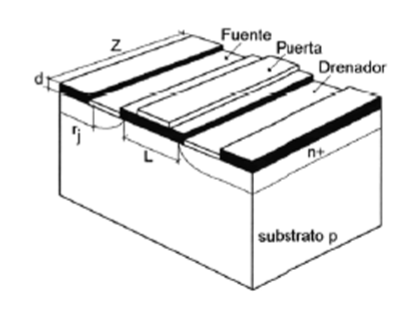
\includegraphics[width=0.5\linewidth]{Imagenes/Tecnologia de CI - MOSFTE.png}
\end{figure}

La tecnología MOSFET se divide en N-MOS, P-MOS y C-MOS. Los parámetros importantes del MOSFET son:

\begin{itemize}
    \item Longitud del canal (L)
    \item Anchura del canal (Z)
    \item Espesor de óxido (d)
    \item Profundidad de la unión (rj)
    \item Dopaje del semiconductor (ND)
\end{itemize}

\subsection{Empaquetado de Circuitos Integrados}

Las obleas son cortadas para poder extraer cada uno de los chips que la componen. Con un dispositivo de succión, los chips son separados de la oblea y transferidos al lead-frame donde es adhesivado.

El lead-frame es la estructura metálica sobre la que se fija el circuito integrado. Dipone de las patillas que finalmente se utilizan para el montaje en la PCI y posterior soldadura (tanto TH como SMT).

\subsubsection{Wire Bonding}

\begin{figure}[H]
    \centering
    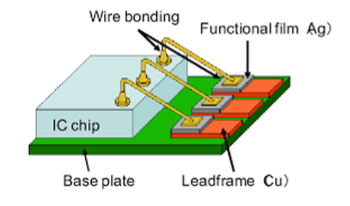
\includegraphics[width=0.5\linewidth]{Imagenes/Tecnologia de CI - Wire Bonding.png}
\end{figure}

El wire bonding es una técnica de conexión de los terminales del CI al lead frame. Esta se realiza por termocompresión de un hilo de oro, plata ó aluminio.

Esta técnica es utilizada tambi´ne para el Chip-on-board en la que el circuito integrado se conecta directamente a la PCI. Esto se utiliza en CI de gran densidad de patillas. Permite eliminar el encapsulado ahorrando espacio en la PCI. El acabado final requiere el recubrimiento con resina epoxy, para protegerlo físicamente y aislarlo eléctricamente.

\subsubsection{Encapsulados}
 Los empaquetados de circuitos integrados pueden ser plásticos (resina) moldeada ó depositada y cerámicos. Los hay para formatos de ensamblado tradicional ó de montaje superficial. Diferenciamos de tipo periféricos, con terminales en los laterales del chip (DIL ó QFP), y de tipo grid array, con terminales en la superficie inferior del chip (PGA ó BGA).